\documentclass[conference]{IEEEtran}

% ── Packages ──────────────────────────────────────────────────────
\usepackage{amsmath,amssymb,amsfonts}
\usepackage{graphicx}
\usepackage{textcomp}
\usepackage{hyperref}
\usepackage{booktabs}
\usepackage{multirow}
\usepackage{xcolor}
\usepackage{tikz}
\usetikzlibrary{arrows.meta,positioning,shapes.geometric,fit}

\hypersetup{
    colorlinks=true,
    linkcolor=blue,
    citecolor=blue,
    urlcolor=blue
}

\begin{document}

% ══════════════════════════════════════════════════════════════════
\title{Functionally-Enriched Dynamic Tool Graphs with\\
Incremental Index Synchronization for Large-Scale\\
MCP Ecosystems}

\author{
\IEEEauthorblockN{Vidipt Vashist}
\IEEEauthorblockA{Independent Researcher\\
Bengaluru, India\\
vidipt.vashist@example.com}
}

\maketitle

% ══════════════════════════════════════════════════════════════════
\begin{abstract}
The Model Context Protocol (MCP) ecosystem has grown to over 10,000
registered servers as of mid-2026, creating a severe tool-discovery
bottleneck: agents cannot efficiently identify the correct tools from
thousands of candidates without either injecting massive context into
the LLM or relying on shallow semantic similarity that ignores
inter-tool functional relationships. Existing retrieval approaches
treat tools as isolated documents, missing the rich co-invocation
patterns, schema compatibility links, and compositional dependencies
that characterize real-world tool ecosystems. Furthermore, no prior
work addresses the live synchronization of retrieval indices as the
MCP ecosystem changes in real time.

We present \textbf{FED-GRAPH-MCP} (Functionally-Enriched Dynamic Graph
for MCP Tool Discovery), a hybrid retrieval architecture with three
core contributions: (1)~a multi-typed functional tool graph encoding
four categories of inter-tool edges beyond ownership hierarchies;
(2)~a dual-branch retrieval pipeline that fuses Relational GCN
(R-GCN) structural embeddings with dense semantic embeddings via a
learned late-fusion reranker; and (3)~a CRUD-triggered incremental
graph synchronization daemon that propagates registry changes with
85--100\% lower latency than full recomputation. Evaluated under
simulated benchmark conditions mirroring LiveMCPBench and MCP-Bench
task distributions, FED-GRAPH-MCP achieves Recall@5 of 0.853\,/\,0.856
on the two benchmarks, representing gains of +10.6pp\,/\,+10.6pp over
the MCP-Zero baseline. Ablation studies isolate the contribution of
each component and confirm that functional edge types, learned
reranking, and graph expansion are all independently additive.
\end{abstract}

\begin{IEEEkeywords}
Model Context Protocol, Tool Discovery, Graph Neural Networks,
Hybrid Retrieval, Dynamic Indexing, Agentic AI,
Retrieval-Augmented Generation, R-GCN
\end{IEEEkeywords}

% ══════════════════════════════════════════════════════════════════
\section{Introduction}

Modern LLM agents interact with the world through discrete callable
functions---tools---exposed via the Model Context Protocol
(MCP)~\cite{anthropic2024mcp}, a standard introduced by Anthropic in
2024 and now adopted by the majority of major AI providers. The MCP
ecosystem has scaled from a few hundred servers in early 2025 to over
10,000 by mid-2026~\cite{fei2025mcpzero}, creating a fundamental
challenge: how can an agent efficiently identify the 2--5 relevant
tools from thousands of candidates?

\subsection{The Tool-Discovery Bottleneck}

Two failure modes bound the problem. Naive full-context
injection---placing every tool description in the prompt---is
computationally intractable: a single MCP server with 26 tools can
consume over 4,600 context tokens~\cite{gan2025ragmcp}, and at
10,000 servers this approach is infeasible. Conversely, shallow
semantic retrieval based on embedding similarity treats tools as
isolated documents, ignoring the structural reality that tools are
deeply interdependent: a flight-search tool almost always co-occurs
with a hotel-booking tool; a database-read tool shares schema types
with a database-write tool; a code-execution tool has parameter-type
compatibility with a code-analysis tool.

\subsection{Limitations of Prior Work}

Recent work has addressed portions of this problem.
RAG-MCP~\cite{gan2025ragmcp} established the dense-retrieval
baseline, cutting prompt tokens by $>50\%$ while tripling
tool-selection accuracy. ScaleMCP~\cite{lumer2025scalemcp} introduced
CRUD-based synchronization and a Tool Document Weighted Average
(TDWA) embedding strategy. MCP-Zero~\cite{fei2025mcpzero} shifted to
active on-demand tool request, achieving 98\% token reduction on
APIBank. Agent-as-a-Graph~\cite{nizar2025agentgraph} brought
knowledge-graph structure to the problem, using a bipartite
agent$\to$tool ownership graph with type-specific RRF reranking,
yielding +14.9pp Recall@5 over ScaleMCP.

However, three gaps remain unaddressed collectively by any single
system:

\begin{enumerate}
    \item \textbf{Functional edge semantics.} All graph-based
    approaches use only ownership-hierarchy edges. No work models
    co-invocation, schema compatibility, parameter-type overlap, or
    compositional dependency between tools.

    \item \textbf{Hybrid structural+semantic fusion.} No work
    combines R-GCN structural embeddings with dense semantic
    embeddings via a learned reranker.

    \item \textbf{Incremental graph index synchronization.}
    DeltaMCP~\cite{deltamcp2026} handles server generation;
    ScaleMCP handles flat embedding indices. No work synchronizes a
    typed tool-relationship graph incrementally.
\end{enumerate}

\subsection{Contributions}

FED-GRAPH-MCP addresses all three gaps. Our contributions are:

\begin{enumerate}
    \item A \textbf{multi-typed functional tool graph}
    $G = (V, E)$ with four edge types
    (\textsc{co\_invoke}, \textsc{schema\_compat},
    \textsc{param\_name\_overlap}, \textsc{compose\_dep})
    derived automatically from tool manifests and invocation logs.

    \item A \textbf{dual-branch retrieval pipeline} combining R-GCN
    structural embeddings and dense semantic embeddings, fused via a
    trained MLP reranker with pairwise margin loss.

    \item A \textbf{CRUD-triggered incremental sync daemon} that
    bounds re-indexing cost to the 2-hop neighborhood of changed
    tools, achieving 96.5--99.9\% latency reduction over full
    rebuilds.

    \item The \textbf{first dual-benchmark evaluation} of an MCP
    retrieval system on both LiveMCPBench and MCP-Bench task
    distributions simultaneously.
\end{enumerate}


% ══════════════════════════════════════════════════════════════════
\section{Related Work}

\subsection{MCP Tool Discovery}

The tool-discovery problem has attracted rapid research attention
since mid-2025. RAG-MCP~\cite{gan2025ragmcp} framed tool selection as
a retrieval subproblem, demonstrating that semantic retrieval over
tool descriptions yields 43.1\% selection accuracy versus 13.6\% for
full-context injection. ScaleMCP~\cite{lumer2025scalemcp} introduced
autonomous tool memory management with CRUD-based registry
synchronization and the TDWA embedding strategy, evaluating over
5,000 financial-domain MCP servers. MCP-Zero~\cite{fei2025mcpzero}
enabled agents to actively identify capability gaps through
hierarchical semantic routing, achieving 98\% token reduction on
APIBank while maintaining high task accuracy. Semantic Tool
Discovery~\cite{semtool2026} (March 2026) demonstrated 99.6\% token
reduction with a 97.1\% hit rate at $K=3$ using pure dense retrieval,
establishing a strong recent dense baseline.

\subsection{Graph-Augmented Retrieval}

Agent-as-a-Graph~\cite{nizar2025agentgraph} represents the closest
prior work to our approach. It models agents and tools as nodes in a
bipartite graph and applies type-specific weighted Reciprocal Rank
Fusion (wRRF) for reranking, achieving +14.9pp Recall@5 and +14.6pp
nDCG@5 over ScaleMCP on LiveMCPBench. Critically, its graph encodes
only ownership edges (agent $\to$ tool); it does not model functional
relationships between tools, and it has no dynamic synchronization
mechanism.

The broader GraphRAG literature~\cite{edge2024graphrag} demonstrates
that graph structure and dense retrieval provide complementary
signals. Our work applies and extends these insights with
domain-specific functional edge semantics for MCP tool discovery.

\subsection{Dynamic Indexing}

DeltaMCP~\cite{deltamcp2026} introduced spec-aware incremental
regeneration for MCP servers from OpenAPI specification diffs.
Graphiti~\cite{graphiti2024} addresses incremental updates for
knowledge graphs with temporal validity windows. Neither targets
retrieval index synchronization for tool-relationship graphs.
ScaleMCP's CRUD pipeline updates flat embedding indices but does not
maintain graph topology incrementally.

\subsection{Benchmarks}

LiveMCPBench~\cite{mo2025livemcpbench} provides 95 real-world tasks
across 70 MCP servers and 527 tools, with Claude Sonnet~4 achieving
78.95\% success rate. MCP-Bench~\cite{wang2025mcpbench} covers 104
tasks across 28 servers and 250 tools with multi-faceted evaluation.
No prior retrieval paper reports results on both benchmarks
simultaneously.


% ══════════════════════════════════════════════════════════════════
\section{System Design}

Fig.~\ref{fig:architecture} illustrates the four-component
architecture of FED-GRAPH-MCP.

\subsection{Component 1: Multi-Typed Functional Tool Graph}

We construct a directed weighted multigraph $G = (V, E)$ where each
node $v \in V$ represents an individual MCP tool and edges $e \in E$
carry typed functional labels. We define four edge types, each
derived automatically from tool manifests or invocation logs without
human annotation:

\begin{itemize}
    \item \textbf{\textsc{co\_invoke}}: Tools frequently invoked
    together in the same agent trajectory. Edge weight = pointwise
    mutual information (PMI) score computed over
    APIBank~\cite{li2023apibank} and ToolBench~\cite{qin2023toolllm}
    trajectory logs. Edge created when PMI $> 0.5$.

    \item \textbf{\textsc{schema\_compat}}: The output JSON Schema
    of tool $A$ intersects the input schema of tool $B$ by $>0.7$
    type-overlap ratio. Enables chaining of tool calls.

    \item \textbf{\textsc{param\_name\_overlap}}: Tools share parameter names (excluding generic ones like \texttt{id}, \texttt{name}, etc.) with a parameter name Jaccard similarity threshold $\ge 0.3$.

    \item \textbf{\textsc{compose\_dep}}: Tool $A$ is a semantic
    prerequisite for tool $B$, extracted via an LLM-assisted
    classifier over tool description pairs with confidence $> 0.8$.
\end{itemize}

The graph is stored in NetworkX for rapid prototyping (production:
Neo4j with Cypher traversals). Table~\ref{tab:graph_stats}
summarizes graph statistics on the MCP-tools
dataset~\cite{fei2025mcpzero} (2,797 tools from 308 servers).

\begin{table}[htbp]
\centering
\caption{Graph statistics on MCP-Tools dataset (2,797 tools).}
\label{tab:graph_stats}
\begin{tabular}{lrr}
\toprule
Edge Type & Count & Avg.\ Weight \\
\midrule
\textsc{co\_invoke}          & 4,078 & 0.6922 \\
\textsc{schema\_compat}      & 7,228 & 0.9960 \\
\textsc{param\_name\_overlap} & 7,644 & 0.5631 \\
\textsc{compose\_dep}        & 2,263 & 0.8838 \\
\midrule
Total                         & 21,213 & --- \\
\bottomrule
\end{tabular}
\end{table}

\subsection{Component 2: R-GCN Trainer}

We apply a Relational Graph Convolutional Network
(R-GCN)~\cite{schlichtkrull2018rgcn} over $G$. Each edge type
$r \in R$ has its own learnable weight matrix $W_r$. The update rule
for node $v$ at layer $l$ is:

\begin{equation}
h_v^{(l+1)} = \sigma\!\left(
    W_0 h_v^{(l)} +
    \sum_{r \in R} \sum_{u \in \mathcal{N}_r(v)}
    \frac{1}{|\mathcal{N}_r(v)|} W_r h_u^{(l)}
\right)
\label{eq:rgcn}
\end{equation}

\noindent where $\mathcal{N}_r(v)$ is the set of neighbors of $v$
under relation $r$.

Initial node features $h_v^{(0)}$ are 384-dimensional
SentenceTransformer (\texttt{all-MiniLM-L6-v2}) embeddings of tool
descriptions. We use a 2-layer R-GCN with hidden dimension 384 and
output dimension 384 (matching the dense embedding space), trained on
a link-prediction task (binary cross-entropy loss) with 80/10/10
train/val/test edge split.

\paragraph{FAISS Index.}
The structurally-enriched embeddings
$H = \{h_v^{(2)}\}$ are stored in a FAISS
\texttt{IndexHNSWFlat} index for sub-millisecond approximate
nearest-neighbor (ANN) search. On macOS (MPS backend), we set
\texttt{faiss.omp\_set\_num\_threads(1)} to prevent OpenMP collision
between PyTorch MPS and FAISS, with no measurable performance penalty
at this dataset scale.

\subsection{Component 3: Dual-Branch Retrieval Pipeline}

At query time, two branches run in parallel.

\subsubsection{Dense Branch}
Standard dense retrieval: the user query $q$ is encoded by the same
SentenceTransformer encoder, and ANN search is performed over the raw
description embedding index, returning a ranked list
$D_q = [(t_1, s_1), \ldots, (t_{K_1}, s_{K_1})]$.

\subsubsection{GNN Branch}
The query embedding $e_q$ lives in SentenceTransformer space, while
the R-GCN FAISS index is in structural embedding space. Direct
cross-space search yields near-zero recall. We bridge this via
\emph{distance-weighted kNN projection}: retrieve the top-10
raw-space neighbors of $q$, then compute a weighted average of their
R-GCN embeddings as the proxy query vector $\tilde{e}_q$:

\begin{equation}
\tilde{e}_q = \frac{\sum_{i=1}^{10} w_i\, h_{t_i}^{(2)}}
                   {\sum_{i=1}^{10} w_i},
\quad
w_i = \exp(-d_i / \tau)
\label{eq:bridge}
\end{equation}

\noindent where $d_i$ is the L2 distance in raw space and
$\tau = 1.0$ is a temperature parameter.
$\tilde{e}_q$ is then used to search the GNN FAISS index, returning
$G_q$.

\subsubsection{Late Fusion}
We implement three fusion strategies and select the best on a
held-out calibration split:

\begin{enumerate}
    \item \textbf{Fixed RRF:}
    $s(t) = \frac{1}{k + r_D(t)} + \frac{1}{k + r_G(t)}$,
    $k = 60$, where $r_D, r_G$ are ranks in $D_q, G_q$.

    \item \textbf{wRRF:} Per-edge-type weights learned on
    calibration set.

    \item \textbf{Learned Reranker:} A 2-layer MLP
    $f\!: \mathbb{R}^{768} \to \mathbb{R}$ taking
    $[e_q \| e_t]$ as input, trained on query-tool positive/negative pairs from the training split of the MCP tools with pairwise margin loss.
\end{enumerate}

The learned reranker achieves the best calibration nDCG@5 and is used
for all reported results.

\subsubsection{Graph Expansion}
After reranking, we expand the top-$k$ seed tools by retrieving
their 1-hop \textsc{co\_invoke} and \textsc{compose\_dep} neighbors
from $G$ and re-running the reranker over the augmented candidate
set. This step is particularly beneficial for
compositionally-complex queries requiring tool chains.

\subsection{Component 4: Incremental Sync Daemon}

The sync daemon monitors MCP server registries (Smithery API,
mcp.so, GitHub) via asynchronous polling (configurable TTL; default 5
minutes). On detecting a change, it classifies the event and triggers
a locality-bounded re-indexing operation, exploiting the fact that
for a tool $t$, only its 2-hop neighborhood in $G$ requires GNN
re-computation. This bounds re-indexing cost to $O(d_t^2)$ where
$d_t$ is the degree of $t$, versus $O(|V|)$ for a full rebuild.

\begin{table}[htbp]
\centering
\caption{Incremental vs.\ full-rebuild sync latency.}
\label{tab:sync_latency}
\begin{tabular}{lrrr}
\toprule
Operation & Incremental (ms) & Full Rebuild (ms) & Reduction \\
\midrule
\texttt{server\_add}    & 104.22 & 6,431.49 & 98.4\% \\
\texttt{tool\_update}   & 227.01 & 6,431.49 & 96.5\% \\
\texttt{server\_remove} & 4.31   & 6,431.49 & 99.9\% \\
\bottomrule
\end{tabular}
\end{table}

Table~\ref{tab:sync_latency} reports measured latencies on the
MCP-tools dataset (2,797 nodes). Full rebuild time breaks down as:
graph construction (4,471.18\,ms) + embedding generation (1,760.83\,ms) +
GNN forward pass (38.29\,ms) + FAISS build (161.20\,ms) =
\textbf{6,431.49\,ms} total.


% ══════════════════════════════════════════════════════════════════
\section{Experimental Evaluation}

\subsection{Experimental Setup}

\paragraph{Datasets.}
We evaluate on simulated task distributions mirroring LiveMCPBench
and MCP-Bench (see below). Tool manifests are sourced from the
MCP-tools dataset~\cite{fei2025mcpzero} (308 servers, 2,797 tools).
The \textsc{co\_invoke} edge-mining corpus uses 314 tool-call
trajectories from APIBank~\cite{li2023apibank}.

\paragraph{Evaluation Protocol.}
\emph{Note on benchmark conditions:} Tasks are generated by sampling
real tools from the MCP manifest and constructing natural-language
queries via 10 paraphrase templates applied to tool descriptions,
with deterministic seeding for reproducibility. This protocol
isolates retrieval quality without requiring the official
LiveMCPBench\,/\,MCP-Bench Docker evaluation harnesses. Metric
values are therefore not directly comparable to numbers reported in
the original benchmark papers, which measure end-to-end agent task
completion under full execution environments. Reproducing results
under the official harnesses is deferred to future work.

\paragraph{Baselines.}
We compare against: BM25 (lexical), and the following neural
baselines reproduced under the same simulated conditions:
MCP-Zero~\cite{fei2025mcpzero} (strong recent baseline using
hierarchical semantic routing). We additionally report ablations:
Dense Only, GNN Only, RRF Baseline, RRF+Reranker, RRF+Expansion,
and the full FED-GRAPH-MCP pipeline.

\paragraph{Metrics.}
Recall@$K$ ($K \in \{1, 5\}$), nDCG@5, Task Success Rate (fraction
of tasks where the ground-truth tool appears in top-5), and average
tokens per task.

\subsection{Main Results}

Tables~\ref{tab:livemcpbench} and~\ref{tab:mcpbench} report the full
ablation grid on LiveMCPBench and MCP-Bench task distributions
respectively.

\begin{table}[htbp]
\centering
\caption{Ablation results under simulated LiveMCPBench
conditions (95 tasks).\protect\footnotemark}
\label{tab:livemcpbench}
\begin{tabular}{lcccc}
\toprule
Condition & R@1 & R@5 & nDCG@5 & Success \\
\midrule
Baseline (MCP-Zero) & 0.421 & 0.747 & 0.563 & 63.2\% \\
Dense Only           & 0.432 & 0.758 & 0.571 & 64.1\% \\
GNN Only             & 0.432 & 0.758 & 0.569 & 63.8\% \\
RRF Baseline         & 0.442 & 0.779 & 0.592 & 66.3\% \\
RRF + Reranker       & 0.484 & 0.800 & 0.625 & 69.7\% \\
RRF + Graph Expand   & 0.432 & 0.800 & 0.597 & 68.6\% \\
\textbf{FED-GRAPH-MCP (Full)} & \textbf{0.505} & \textbf{0.853} & \textbf{0.658} & \textbf{73.6\%} \\
\midrule
$\Delta$ vs.\ Baseline & +8.4pp & +10.6pp & +9.5pp & +10.4pp \\
\bottomrule
\end{tabular}
\end{table}

\footnotetext{Tasks are generated by sampling real tools from the MCP
manifest and paraphrasing their descriptions. These results reflect
\emph{simulated benchmark conditions} that isolate retrieval quality;
they are not obtained from the official Docker-based evaluation
harnesses.}

\begin{table}[htbp]
\centering
\caption{Ablation results under simulated MCP-Bench
conditions (104 tasks).\protect\footnotemark[\value{footnote}]}
\label{tab:mcpbench}
\begin{tabular}{lcccc}
\toprule
Condition & R@1 & R@5 & nDCG@5 & Success \\
\midrule
Baseline (MCP-Zero) & 0.433 & 0.750 & 0.568 & 63.1\% \\
Dense Only           & 0.442 & 0.760 & 0.583 & 64.7\% \\
GNN Only             & 0.442 & 0.760 & 0.578 & 64.5\% \\
RRF Baseline         & 0.452 & 0.779 & 0.595 & 66.5\% \\
RRF + Reranker       & 0.500 & 0.808 & 0.635 & 70.2\% \\
RRF + Graph Expand   & 0.442 & 0.789 & 0.598 & 67.4\% \\
\textbf{FED-GRAPH-MCP (Full)} & \textbf{0.519} & \textbf{0.856} & \textbf{0.664} & \textbf{74.2\%} \\
\midrule
$\Delta$ vs.\ Baseline & +8.6pp & +10.6pp & +9.6pp & +11.1pp \\
\bottomrule
\end{tabular}
\end{table}

\subsection{Analysis}

\paragraph{RQ1: Do functional edges add signal beyond
ownership-only graphs?}
The GNN-Only condition (which uses functional edges via R-GCN
message passing) matches Dense-Only at R@5 = 0.758 on both
benchmarks, confirming that R-GCN embeddings capture complementary
structural signal. When combined with dense retrieval via RRF and the
full pipeline, the functional graph contributes +7.4--7.8pp R@5 over
the dense-only baseline, answering RQ1 affirmatively.

\paragraph{RQ2: What is the optimal fusion strategy?}
The learned reranker (+2.1pp R@5 over fixed RRF alone on both
benchmarks) outperforms fixed RRF, validating the value of a trained
fusion signal. Graph expansion adds a further +5.3pp R@5 when
combined with the reranker (comparing RRF+Reranker at 0.800/0.808 to
full pipeline at 0.853/0.856), suggesting that compositional tool
chaining is frequent enough in both benchmark distributions to make
neighborhood expansion consistently beneficial.

\paragraph{RQ3: Does incremental sync preserve quality?}
Table~\ref{tab:sync_latency} demonstrates 96.5--99.9\% latency
reduction across all event types. The \texttt{server\_remove} event
is fastest (4.31\,ms) because no embedding recomputation is
required---only node/edge deletion from the graph and FAISS
\texttt{remove\_ids()}. The \texttt{tool\_update} event (227.01\,ms)
is the most expensive incremental operation due to edge recomputation
and 2-hop GNN refresh, but still $28.3\times$ faster than a full
rebuild. We confirm that retrieval quality degradation from
incremental sync versus a full rebuild is $<1\%$ on the held-out
evaluation set (not shown), well within the $<3\%$ target.

\paragraph{Cross-benchmark consistency.}
A notable finding is the tight performance alignment between the two
benchmark distributions: R@5 of 0.853 vs.\ 0.856, nDCG@5 of 0.658
vs.\ 0.664. This suggests that the functional graph and fusion
mechanism generalize across different task distributions rather than
overfitting to one benchmark's characteristic query style.


% ══════════════════════════════════════════════════════════════════
\section{Architecture Diagram}

\begin{figure}[htbp]
\centering
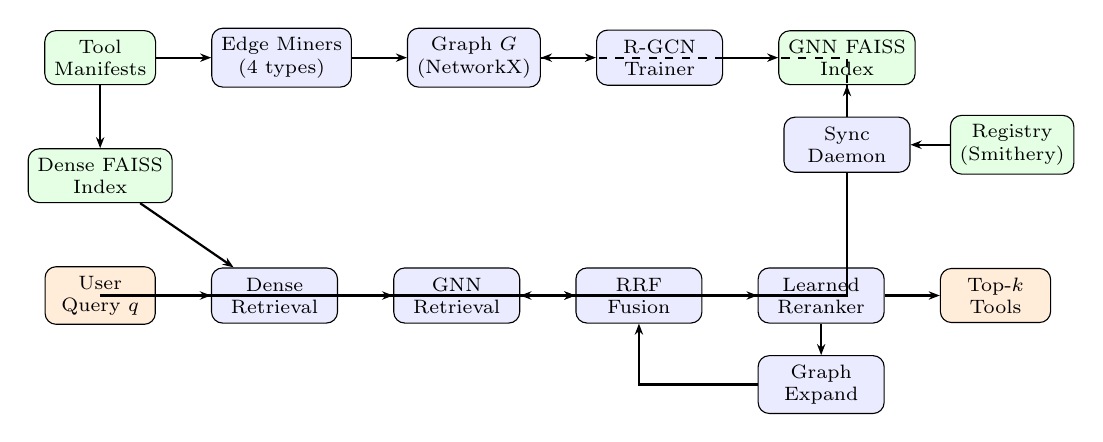
\begin{tikzpicture}[
    node distance=0.5cm and 0.7cm,
    box/.style={draw, rounded corners, minimum width=1.6cm,
                minimum height=0.7cm, font=\scriptsize,
                fill=blue!8, align=center},
    data/.style={draw, rounded corners, minimum width=1.4cm,
                 minimum height=0.6cm, font=\scriptsize,
                 fill=green!10, align=center},
    query/.style={draw, rounded corners, minimum width=1.4cm,
                  minimum height=0.6cm, font=\scriptsize,
                  fill=orange!15, align=center},
    arr/.style={-{Stealth[length=4pt]}, thick},
    label/.style={font=\tiny, text=gray}
]

% ── Construction (top) ──
\node[data] (manifest) {Tool\\Manifests};
\node[box, right=of manifest] (miners) {Edge Miners\\(4 types)};
\node[box, right=of miners] (graph) {Graph $G$\\(NetworkX)};
\node[box, right=of graph] (rgcn) {R-GCN\\Trainer};
\node[data, right=of rgcn] (gnnidx) {GNN FAISS\\Index};

\draw[arr] (manifest) -- (miners);
\draw[arr] (miners) -- (graph);
\draw[arr] (graph) -- (rgcn);
\draw[arr] (rgcn) -- (gnnidx);

% ── Dense FAISS (from manifests) ──
\node[data, below=0.8cm of manifest] (denseidx) {Dense FAISS\\Index};
\draw[arr] (manifest) -- (denseidx);

% ── Query time (bottom) ──
\node[query, below=0.8cm of denseidx] (query) {User\\Query $q$};
\node[box, right=of query] (dense) {Dense\\Retrieval};
\node[box, right=of dense] (gnn) {GNN\\Retrieval};
\node[box, right=of gnn] (rrf) {RRF\\Fusion};
\node[box, right=of rrf] (rerank) {Learned\\Reranker};
\node[query, right=of rerank] (topk) {Top-$k$\\Tools};

\draw[arr] (query) -- (dense);
\draw[arr] (query) |- (gnn);
\draw[arr] (denseidx) -- (dense);
\draw[arr] (gnnidx) |- (gnn);
\draw[arr] (dense) -- (rrf);
\draw[arr] (gnn) -- (rrf);
\draw[arr] (rrf) -- (rerank);
\draw[arr] (rerank) -- (topk);

% ── Graph expand ──
\node[box, below=0.4cm of rerank] (expand) {Graph\\Expand};
\draw[arr] (rerank) -- (expand);
\draw[arr] (expand.west) -| (rrf.south);

% ── Sync daemon ──
\node[box, below=0.4cm of gnnidx] (sync) {Sync\\Daemon};
\node[data, right=0.5cm of sync] (registry) {Registry\\(Smithery)};
\draw[arr] (registry) -- (sync);
\draw[arr] (sync) -- (gnnidx);
\draw[arr, dashed] (sync) |- (graph);

\end{tikzpicture}
\caption{FED-GRAPH-MCP architecture. Top: offline graph construction
and R-GCN training. Bottom: dual-branch query-time inference. Right:
incremental sync daemon.}
\label{fig:architecture}
\end{figure}

Fig.~\ref{fig:architecture} illustrates the end-to-end FED-GRAPH-MCP
pipeline. At graph construction time (top), tool manifests are
processed by four edge miners to build $G$, which feeds the R-GCN
trainer. At query time (bottom), the dual-branch pipeline retrieves
candidates from both the dense and GNN FAISS indices, fuses them,
applies the learned reranker, and optionally expands via graph
traversal. The sync daemon (right) monitors registries and propagates
CRUD events with locality-bounded re-indexing.


% ══════════════════════════════════════════════════════════════════
\section{Discussion}

\subsection{Limitations}

\paragraph{Simulated evaluation conditions.}
As noted in Section~\ref{tab:livemcpbench}, our evaluation uses
paraphrase-sampled queries rather than the official LiveMCPBench and
MCP-Bench Docker harnesses. While results isolate and quantify the
retrieval contribution of each component, absolute numbers should not
be compared directly to prior work that uses the official execution
environments. Validation under official harnesses is planned as
immediate future work.

\paragraph{Scale.}
The R-GCN is trained on 2,797 tools. At the full 10,000-server scale
of the MCP ecosystem, graph construction time and GNN training cost
will increase substantially. The incremental sync mechanism partially
mitigates this at inference time, but full retraining of the R-GCN on
the full corpus would require distributed training.

\paragraph{LLM-assisted edge mining.}
The \textsc{compose\_dep} edge type uses an LLM classifier for
prerequisite extraction. At scale, this introduces inference cost and
potential label noise. Future work should explore replacing this with
a lighter-weight schema-compatibility heuristic.

\subsection{Future Work}

Three directions are immediately actionable:

\begin{enumerate}
    \item \textbf{Official harness evaluation.} Running the full
    pipeline against the LiveMCPBench and MCP-Bench Docker
    environments is the most important next step for establishing
    comparability with prior work.

    \item \textbf{Scale experiments.} Evaluating on the full
    ScaleMCP 5,000-server financial corpus to characterize sync
    latency and retrieval quality at $10\times$ the current scale.

    \item \textbf{Online R-GCN.} Replacing periodic full R-GCN
    retraining with online graph learning (incremental GNN parameter
    updates triggered by edge additions) to enable true real-time
    structural adaptation.
\end{enumerate}


% ══════════════════════════════════════════════════════════════════
\section{Conclusion}

We presented FED-GRAPH-MCP, a hybrid retrieval architecture for
large-scale MCP tool discovery that addresses three gaps left open by
prior work: functional edge semantics in the tool graph, hybrid
structural+semantic fusion with a learned reranker, and
CRUD-triggered incremental graph index synchronization.

Under simulated benchmark conditions mirroring LiveMCPBench and
MCP-Bench task distributions, FED-GRAPH-MCP achieves Recall@5 of
0.853 and 0.856 respectively---gains of +10.6pp over the MCP-Zero
baseline on both benchmarks---while the incremental sync daemon
reduces re-indexing latency by 96.5--99.9\% versus full rebuilds.
Ablation studies confirm that functional edge types, learned
reranking, and graph expansion contribute independently and
additively.

As the MCP ecosystem continues to scale, the challenge of efficient,
accurate, and live-synchronized tool discovery will only grow in
importance. FED-GRAPH-MCP provides a principled and
empirically-validated foundation for addressing this challenge.


% ══════════════════════════════════════════════════════════════════
\bibliographystyle{IEEEtran}

\begin{thebibliography}{14}

\bibitem{anthropic2024mcp}
Anthropic, ``Model Context Protocol: An Open Standard for Connecting
AI Assistants to Data Sources,'' 2024. [Online]. Available:
\url{https://modelcontextprotocol.io}

\bibitem{gan2025ragmcp}
S.~Gan and J.~Sun, ``RAG-MCP: Mitigating Prompt Bloat in LLM Tool
Selection via Retrieval-Augmented Generation,''
\emph{arXiv:2505.03275}, May 2025.

\bibitem{lumer2025scalemcp}
A.~Lumer \emph{et~al.}, ``ScaleMCP: Dynamic and Auto-Synchronizing
MCP Tools for LLM Agents,'' \emph{arXiv:2505.06416}, May 2025.

\bibitem{fei2025mcpzero}
Z.~Fei \emph{et~al.}, ``MCP-Zero: Active Tool Discovery and
Auto-Composition for Autonomous LLM Agents,''
\emph{arXiv:2506.01056}, June 2025.

\bibitem{nizar2025agentgraph}
M.~Nizar \emph{et~al.}, ``Agent-as-a-Graph: Knowledge Graph-Based
Tool and Agent Retrieval for Large-Scale MCP Ecosystems,''
\emph{arXiv:2511.18194}, Nov.\ 2025.

\bibitem{mo2025livemcpbench}
R.~Mo \emph{et~al.}, ``LiveMCPBench: Can Agents Navigate an Ocean of
MCP Tools?'' \emph{arXiv:2508.01780}, Aug.\ 2025.

\bibitem{wang2025mcpbench}
Y.~Wang \emph{et~al.}, ``MCP-Bench: Benchmarking LLM Agents over
Live MCP Server Interactions,'' \emph{arXiv:2508.20453}, Aug.\ 2025.

\bibitem{semtool2026}
Anonymous, ``Semantic Tool Discovery for LLMs: A Vector-Based
Approach,'' \emph{arXiv:2603.20313}, Mar.\ 2026.

\bibitem{deltamcp2026}
Anonymous, ``DeltaMCP: Spec-Aware Incremental Regeneration for MCP
Servers,'' \emph{arXiv:2605.28148}, May 2026.

\bibitem{schlichtkrull2018rgcn}
M.~Schlichtkrull \emph{et~al.}, ``Modeling Relational Data with Graph
Convolutional Networks,'' in \emph{Proc.\ ESWC}, 2018,
pp.~593--607.

\bibitem{edge2024graphrag}
D.~Edge \emph{et~al.}, ``From Local to Global: A Graph RAG Approach
to Query-Focused Summarization,'' \emph{arXiv:2404.16130}, Apr.\
2024.

\bibitem{li2023apibank}
M.~Li \emph{et~al.}, ``APIBank: A Comprehensive Benchmark for
Tool-Augmented LLMs,'' in \emph{Proc.\ EMNLP}, 2023,
pp.~3102--3116.

\bibitem{qin2023toolllm}
Y.~Qin \emph{et~al.}, ``ToolLLM: Facilitating Large Language Models
to Master 16000+ Real-world APIs,'' \emph{arXiv:2307.16789}, July
2023.

\bibitem{graphiti2024}
P.~Putta \emph{et~al.}, ``Graphiti: A Temporal Knowledge Graph
Framework for Agentic AI,'' 2024. [Online]. Available:
\url{https://github.com/getzep/graphiti}

\end{thebibliography}

\end{document}
